\documentclass{foi}
\usepackage[utf8]{inputenc}
\usepackage{lipsum}
\DeclareUnicodeCharacter{0140}{l}
\vrstaRada{\diplomski} % \diplomski
\title{Izrada komponente za detekciju označenih odgovora na pismenim ispitima}
\author{Filip Milohanović}
\spolStudenta{\musko} % \zensko ili \musko
\mentor{Marko Mijač}
\spolMentora{\musko} % \zensko ili \musko
\godina{2025}
\mjesec{lipanj}
\date{2025}
%\status{redoviti}
\jmbag{0016148270 }
\smjer{Informacijsko i programsko inženjerstvo} % (ili Poslovni sustavi, Ekonomika poduzetništva, Primjena informacijske tehnologije u poslovanju, Informacijsko i programsko inženjerstvo, Baze podataka i baze znanja, Organizacija poslovnih sustava, Informatika u obrazovanju)
\titulaProfesora{Doc. dr. sc.}

\sazetak{Opsega od 100 do 300 riječi. Sažetak upućuje na temu rada, ukratko se iznosi čime se rad bavi, teorijsko-metodološka polazišta, glavne teze i smjer rada te zaključci.}

\kljucneRijeci{riječ; riječ; ...riječ; Obuhvaća 7+/-2 ključna pojma koji su glavni predmet rasprave u radu.}

\begin{document}

\maketitle

\tableofcontents

\pagestyle{plain}
\chapter{Uvod}

U današnjem obrazovnom sustavu nastavnici provode jako puno vremena na radnim zadacima koji ne podižu kvalitetu obrazovanja već su administrativni i često repetitivni poslovi. Jedan od tih zadataka je ocjenjivanje ispita, pogotovo ako se radi o velikoj količini pristupnika testu. Kod testova s izrazito velikom količinom pristupnika se zato koriste ispiti koji uključuju list za odgovore što olakšava ocjenjivanje. Time se značajno ubrzava cijeli proces ocjenjivanja pošto nije potrebno čitati odgovore koji su u različitim formatima i potencijalno na više stranica, ali i dalje ostaje repetitivni dio posla koji uključuje usporedbu odgovora s rješenjima. Kroz ovaj rad bit će prikazana softverska komponenta otvorenog koda koja rješava ovaj problem tako da naspram slike detektira označene odgovore i ocjenjuje ispit.

Kroz ovaj rad istražuje se razne metode za detektiranje označenih odgovora s ciljem izrade komponente visoke preciznosti, prateći metodologiju znanstvenog oblikovanja.

\chapter{Metode i tehnike rada}

S obzirom na to da se radi o temi koja uključuje obradu slike, što zahtijeva opsežno istraživanja, manipulaciju parametrima i testiranje pristupa odlučeno je koristiti inkrementalan pristup razvoju. Prije same izrade rješenja, provedena je minimalno potrebna količina istraživanja, a zatim se ostatak istraživanja odvijao paralelno s razvojem.

Iterativni razvoj rješenja može se podijeliti u pretprocesiranje, izdvajanje relevantnih obilježja slike i na kraju ocjenjivanje testa. Jedna od najvažnijih tehnika tijekom razvoja bila je  vizualizacija svakog koraka obrade slike. To je omogućilo izravan uvid u status i smjer razvoja. Od samog početka omogućen je uvid u mane i prednosti korištenih metoda. Ovo je značajno doprinjelo definiranju budućih razvojnih koraka, poput  dodatnog istraživanja, promjene pristupa i sl. 

Da bi sama vizualizacija bila što učinkovitija korišteno je više različitih ulaznih slika matrice odgovora slikanih u različitim uvjetima. To je omogućilo verifikaciju funkcionalnosti dijelova rješenja na različitim ulaznim podacima od samog početka razvoja, što je značilo da na kraju projekta nije bilo potrebno pokrivati rubne slučajeve jer je rješenje bilo dizajnirano da ih pokriva od početka. 

Rješenje je izrađeno pomoću .NET tehnologije i C\# programskog jezika u obliku biblioteke, što omogućuje drugim rješenjima jednostavnu integraciju koristeći .dll. 

Kroz ovaj rad nije bio cilj razviti vlastitu biblioteku za računalni vid, korištena je jedna od  postojećih biblioteka otvorenog koda. EmguCv je odabran pošto se radi o .NET omotaču za jednu od najpopularnijih biblioteka za računalni vid OpenCV. Osim toga, rješenje omogućuje korisnicima da koriste alternativnu biblioteku s uvjetom da izrade svoju implementaciju odgovarajućih metoda.

\chapter{Razrada teme}

Kroz teoretski dio rada predočit će se cijeli proces detekcije odgovora na pismenim ispitima koristeći obradu slike pomoću računalnog vida. Analizirati će postojeća rješenja ovaog problema koja koriste računalni vidi i alternativne pristupe. 

    Svim ti pristupi imaju isti cilj, a to je izvlačenje relevantnih podataka iz slike, a zatim kreće obrada tih podataka. U kontektu ovog rada to bi značilo da se iz slike moraju izvući podaci o označenim odgovorima za određeno pitanje te se ti podaci uspoređuju sa listom točnih odgovora. 

\section{Digitalna slika }

Za početak važno je razumjeti što su to digitalne slike i koje sve informacije one sadrže. Digitalna slika je zapravo računalna datoteka koja reprezentira fotografiju pomoću piksela. Piksel je zapravo najmanji element slike koji je reprezentiran s 3 kanala boja: Crvena (R), zelena (G), plava (B) u RGB modelu. Postoje i drugi kanali boja sli za potrebe ovog rada fokus će biti RGB modelu.  \cite{DigitalnaSlika}.

Sama boja piksela se određuje kombinacijom vrijednosti iz RGB kanala. Dok je sam broj mogućih boja određen brojem bitova koju svaki RGB kanal može poprimiti. Taj koncept se još naziva dubinom boje (eng. color depth). Na primjer, 24-bitna slika može poprimiti do 16,777,216 unikatnih boja pošto svaki kanal ima 8 bitova \cite{DigitalnaSlika}:

\[
\text{Broj boja} = 2^{8} \times 2^{8} \times 2^{8} = 2^{24} = 16,777,216
\]

S pomoću piksela se također može definirati veličinu slike to jest rezolucija. Rezolucija je sveukupan broj piksela koje neka slika sadrži i izražava se množenjem širine slike sa visinom slike npr. $1920 \times $1080. Obično veća rezolucija znači više detalja na slici. Što se više detalja nalazi na slici to su bolje šanse za izvući korisne informacije sa slike. No naravno da rezolucija sama ne određuje kvalitetu digitalne slike, već veliku ulogu igraju i fizički uvjeti u kojima je slika izrađena. Pod to spada osvjetljenje, čistoća kamere, kvaliteta senzora i sl.

\subsection{Slike u boji}
Većina digitalnih slika koje ljudi danas izrađuju su slike u boju te sadrže sva 3 kanala boje. Za razumijevanje ovog rada potrebno je razumijeti kakve informacije sadrži pojedini kanal boje. Svaki kanal predstavlja jednu primarnu boju poput crvene, zelene ili plave. I svaki piksel poprima za svaki kanal neku vrijednost ovisno o kombinaciji bitova. Za 24-bitnu sliku svaki kanal ima 8 bitova to jest 256 mogućih vrijednosti. 

To znači da u svakom kanalu postoji vrijednost od 0 do 255 koja definira jačinu svjetlosti za tu primarnu boju. Nula bi značila kompletno crna boja dok bi 255 bila potpuno osvijetljena primarna boja ovisno o kojem se kanalu radi. Kombinacijom tih 3 kanala se zapravo dobivaju međuboje i time se stvara konačni izgled slike. No osim slika u boji postoje i sive slike. \cite{GrayscaleSlika}. 

\begin{figure}[h!]
    \centering
    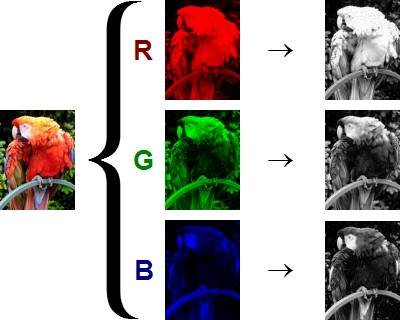
\includegraphics[width=0.5\linewidth]{slike/rgb_channels.png}
    \caption{Prikaz slike u boji i pripadajućih kanala boja u rgb modelu \cite{wikimediaRGB}}
    \label{fig:enter-label}
\end{figure}

Kao što je prikazano na slici, kanali boja prikazani su kao slike čiji pikseli poprimaju boje samo crnu, bijelu i nijanse sive boje, takozvane sive slike. Također kanali se ponekad znaju vizualizirati pomoću primarne boje kanala kojeg reprezentiraju, ali sami podaci koje digitalna slika sadrži su uvijek jednaki, jedino način njihove vizualuizacije varira. 

\subsection{Sive slike}

Sive slike (\textit{eng. grayscale}) su poseban tip digitalnih slika koji ima samo jedan kanal boja. U tom kanalu vrijednosti piksela reprezentira svijetlinu piksela. Vizualizacija takvih slika većinom poprima boje od bijele do crne uključujući nijanse sive. Na primjer za sliku sa dubinom boja od 8 bitova, nula bi predstavljala crnu boju, a 255 bijelu.

Sive slike su jedan od najvažnijih koncepata u obradi slike pošto imaju samo jedan kanal koji opisuje intenzitet svjetlosti, no to ćemo detaljnije prikazati u nastavku \cite{GrayscaleSlika}.

Osim slika u boji i sivih slika također postoje i binarne slike. Binarne slike su tip slika gdje piksel može imati samo dvije moguću vrijednosti 0 i 1 od kud im dolazi i naziv. Binarne slike sadrže puno manje informacija od ostalih tipova slika, ali isto tako smanjuju kompleksnost same slike i omogućuju fokusiranje na važne značajke slike. Baš zbog toga se jako često koriste kod obrada slika koristeći računalni vid \cite{}.


\begin{figure}[h!]
    \centering
    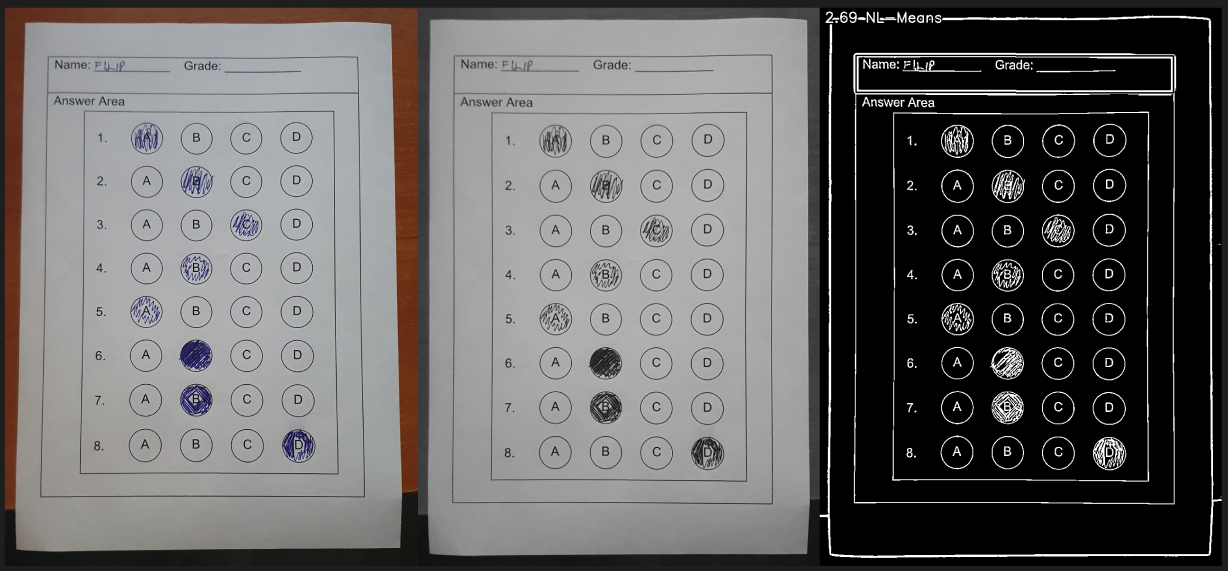
\includegraphics[width=1\linewidth]{slike/usporedbaTipovaSlika.png}
    \caption{Usporedba slike u boji, sive i binarne slike (Vlastita izrada)}
    \label{fig:enter-label}
\end{figure}

\subsection{Poglavlje treće razine}

\lipsum[2]

\subsubsection{Poglavlje četvrte razine}

\lipsum[3-4]

\chapter{Tehničke upute}

Tehničke upute u nastavku opisuju način tehničkog oblikovanja rada i navođenja literature.

\section{Upute za oblikovanje izgleda rada}

\begin{flushleft}\textbf{Stranice} se oblikuju korištenjem sljedećih parametara:\end{flushleft}

\begin{itemize}
    \item veličina i oblik papira je A4, okomito usmjerenje, margine 2,5 cm na svakoj strani;

    \item naslovna stranica rada se ne numerira;

    \item nakon naslovne stranice, sve sljedeće stranice do 1. Poglavlja se numeriraju rimskim brojevima, počevši od i;

    \item od 1. poglavlja nadalje, stranice se numeriraju arapskim brojevima;

    \item broj stranice treba pozicionirati desno 1,25 cm od dna stranice, font Arial 9.
\end{itemize}
\begin{flushleft}\textbf{Tekst} rada je potrebno oblikovati sukladno ovom predlošku, odnosno na sljedeći način:\end{flushleft}
\begin{itemize}
    \item u pisanju teksta koristite font Arial 11 pt, s proredom 1,5 te razmakom 0 pt prije i razmakom 6 pt poslije odlomka, pri čemu je prvi redak uvučen za 1,25 cm;

    \item u naslovima prve razine „3. Razrada teme“ koristite font Arial 18 pt, podebljano, prijelom stranice (svaki naslov prve razine treba biti na novoj stranici), s proredom 1,5 te razmakom 0 pt prije i razmakom 18 pt poslije odlomka;

    \item u naslovima druge razine „2.1. Naslov“ koristite font Arial 16 pt, podebljano, s proredom 1,5 te razmakom 18 pt prije i razmakom 12 pt poslije odlomka;

    \item u naslovima treće razine „2.1.1. Naslov“ koristite font Arial 14 pt, podebljano, s proredom 1,5 te razmakom 12 pt prije i razmakom 6 pt poslije odlomka;

    \item u naslovima četvrte razine „2.1.1.1. Naslov“ koristite font Arial 12 pt, podebljano, s proredom 1,5 te razmakom 6 pt prije i razmakom 6 pt poslije odlomka;

    \item ostalo značajno isticanje cjelina rada može biti istaknuto podebljanim i kurziv slovima, korištenjem fonta Arial 11 pt.
\end{itemize}


\begin{flushleft}\textbf{Slike} u radu je potrebno oblikovati na sljedeći način:
naziv slike navedite ispod slike uz numeraciju;\end{flushleft}

\begin{itemize}
    \item za nazive slika koristite iste postavke fonta kao i za tekst, ali stavite naziv slike u centrirani položaj;

    \item za oblikovanje same slike koristite font Arial 9 pt za tekst na slici;
ispred same slike umetnite jedan prazan redak (osim ako je slika pozicionirana na početku stranice);

    \item nakon naziva slike ostavite jedan redak prazan (osim ako je naziv slike zadnji redak na stranici);

    \item kod prijeloma stranice treba obratiti posebnu pozornost da naziv slike, izvor i sama slika moraju biti na istoj stranici; 

    \item slike je potrebno numerirati redom pojavljivanja u tekstu;

    \item ako je slika preuzeta iz drugog izvora, nakon navođenja naziva slike u zagradi navedite izvor, npr. (autor/autorica, godina);

    \item dozvoljeno je napraviti vlastitu preradu slika, grafikona ili tablica na način da se zadrži isti smisao sadržaja, ali promijeni izgled. I u takvim se slučajevima obavezno u nazivu navodi referenca izvornog djela ovako: “(Prema: Klačmer Čalopa i Cingula, 2012)“;

    \item dozvoljeno je preuzeti samo jednu sliku, grafikon ili tablicu u izvornom obliku iz istog izvora. Za doslovno preuzimanje većeg dijela sadržaja potrebno je ishoditi dozvolu nositelja autorskih prava;

    \item primjer označavanja slike možete vidjeti u nastavku (slika \ref{fig:podjela}).
\end{itemize}

\begin{figure}[h!]
    \centering
    
\includegraphics[width=0.9\textwidth]{slike/slika.png}
    \caption{Podjela investicijskih fondova (Izvor: \citeauthor{Aranda2009}, \citeyear{Aranda2009})}
    \label{fig:podjela}
\end{figure}

\begin{flushleft}\textbf{Tablice} rada je potrebno oblikovati sukladno ovim uputama:\end{flushleft}
\begin{itemize}
    \item naziv tablice navedite iznad slike;

    \item za nazive tablica koristite iste postavke fonta kao i za tekst, ali stavite naziv tablice u centrirani položaj;

    \item za oblikovanje same tablice koristite font Arial 9 pt za tekst u tablici;

    \item tablice numerirajte redom pojavljivanja u tekstu;

    \item prije naziva tablice umetnite jedan redak prazan (osim ako je naziv tablice prvi redak na stranici);

    \item nakon same tablice umetnite jedan prazan redak (osim ako je tablica pozicionirana na kraju stranice);

    \item kod prijeloma stranice treba obratiti posebnu pozornost da naziv tablice, izvor i sama tablica moraju biti na istoj stranici; 

    \item ako je tablica preuzeta iz drugog izvora, nakon navođenja naziva tablice potrebno je navesti izvor, na isti način kako je opisano kod slika;

    \item primjer označavanja tablice možete vidjeti u nastavku (tablica \ref{tab:objekti}).
\end{itemize}

\begin{table}[h!] 
    \centering
    \caption{Prikaz podataka o učestalosti pojavljivanja objekta}
    \begin{tabularx}{0.66\textwidth}{|X|X|X|X|}
        \hline
         \cellcolor{gray!25} & \cellcolor{gray!25} & \cellcolor{gray!25} & \cellcolor{gray!25} \\
        \hline
         &  &  &  \\
        \hline
         &  &  & \\
        \hline
    \end{tabularx}
    \\[10pt]
    \caption*{(Izvor: \citeauthor{caragliu2011smart}, \citeyear{caragliu2011smart})}
    \label{tab:objekti}
\end{table}

\begin{flushleft}\textbf{Programski kod}\end{flushleft}
\begin{itemize}
    \item za oblikovanje teksta koji je programski kôd koristite font Courier, veličine 10 pt, jednostruki prored, 6 pt iza odlomka, npr. HTML kôd dijela zaglavlja početne web stranice FOI weba:
\end{itemize}

\begin{lstlisting}[language=HTML]
<head>
  <meta http-equiv="Content-Type" content="text/html; charset=utf-8" />
  <link rel="shortcut icon" href="https://www.foi.unizg.hr/sites/default/files/favicon_0_1.ico" type="image/vnd.microsoft.icon" />
  <meta name="generator" content="Drupal 7 (http://drupal.org)" />
  <link rel="canonical" href="https://www.foi.unizg.hr/hr" />
  <link rel="shortlink" href="https://www.foi.unizg.hr/hr" />
  <!-- Set the viewport width to device width for mobile -->
  <meta name="viewport" content="width=device-width, initial-scale=1.0">
  <title>Dobro %*došli*) na FOI | FOI</title>...
</head>
\end{lstlisting}

\begin{flushleft}\textbf{Formule}\end{flushleft}
\begin{itemize}
    \item za unos formula koristite editor za formule u svom tekst procesoru.
\end{itemize}

\begin{flushleft}\textbf{Kratice}\end{flushleft}   
\begin{itemize}
    \item ako želite koristiti kratice pojmova u tekstu, kad prvi put spominjete pojam potrebno je navesti puni naziv, a kraticu navesti u zagradi (npr. Informacijske i komunikacijske tehnologije, kraće IKT). Nakon toga možete koristiti kratice u tekstu. Poželjno je u naslovima koristiti pune nazive.
\end{itemize}

\begin{flushleft}\textbf{Strano nazivlje}\end{flushleft}   
\begin{itemize}
    \item strano nazivlje se u tekstu navodi u zagradi, napisano \textit{kurzivom}, nakon hrvatskog izraza, npr. Analiza društvene mreže (engl. \textit{Social Network Analysis - SNA}).
\end{itemize}

\section{Navođenje literature}

Za navođenje literature u radu možete odabrati i koristiti jedan od sljedeća dva ponuđena stila: \textbf{APA} ili \textbf{IEEE} stil. Važno je samo dosljedno primjenjivati odabrani stil u cijelom radu.

U popisu literature potrebno je navesti svu literaturu i samo literaturu koju ste koristili u tekstu.

Uz svaku preuzetu tvrdnju potrebno je navesti njezin izvor, tj. referencu. Reference se u tekstu navode tako da se uz citirani tekst navede izvor, sukladno načinu propisanom odabranim stilom i FOI preporukama za citiranje i referenciranje \cite{SchattenEtAl2016roadmap}.

\chapter{Zaključak}

Ovdje treba sažeto rezimirati najvažnije rezultate razrade teme rada. Potrebno je sažeto opisati što je predmet rada, koje su metode, tehnike, programski alati ili aplikacije korištene u razradi rada te koje su pretpostavke dokazane, a koje opovrgnute. Sadržajno, ono što se u uvodu rada najavljuje i kasnije je obuhvaćeno u samom radu, moralo bi biti opisano u zaključnom dijelu kroz rezultate rada. 

\lipsum[1-2]

\printbibliography[title=Popis literature]
\addcontentsline{toc}{chapter}{Popis literature}

\listoffigures
\addcontentsline{toc}{chapter}{Popis slika}
 
\listoftables
\addcontentsline{toc}{chapter}{Popis popis tablica}

\appendix
\renewcommand{\thechapter}{\arabic{chapter}}

\chapter{Prilog 1}

\chapter{Prilog 2}

\end{document}
